% Options for packages loaded elsewhere
\PassOptionsToPackage{unicode}{hyperref}
\PassOptionsToPackage{hyphens}{url}
%
\documentclass[
]{book}
\usepackage{amsmath,amssymb}
\usepackage{lmodern}
\usepackage{ifxetex,ifluatex}
\ifnum 0\ifxetex 1\fi\ifluatex 1\fi=0 % if pdftex
  \usepackage[T1]{fontenc}
  \usepackage[utf8]{inputenc}
  \usepackage{textcomp} % provide euro and other symbols
\else % if luatex or xetex
  \usepackage{unicode-math}
  \defaultfontfeatures{Scale=MatchLowercase}
  \defaultfontfeatures[\rmfamily]{Ligatures=TeX,Scale=1}
\fi
% Use upquote if available, for straight quotes in verbatim environments
\IfFileExists{upquote.sty}{\usepackage{upquote}}{}
\IfFileExists{microtype.sty}{% use microtype if available
  \usepackage[]{microtype}
  \UseMicrotypeSet[protrusion]{basicmath} % disable protrusion for tt fonts
}{}
\makeatletter
\@ifundefined{KOMAClassName}{% if non-KOMA class
  \IfFileExists{parskip.sty}{%
    \usepackage{parskip}
  }{% else
    \setlength{\parindent}{0pt}
    \setlength{\parskip}{6pt plus 2pt minus 1pt}}
}{% if KOMA class
  \KOMAoptions{parskip=half}}
\makeatother
\usepackage{xcolor}
\IfFileExists{xurl.sty}{\usepackage{xurl}}{} % add URL line breaks if available
\IfFileExists{bookmark.sty}{\usepackage{bookmark}}{\usepackage{hyperref}}
\hypersetup{
  pdftitle={Mappeeksamen},
  pdfauthor={Håvard C. Lorentzen},
  hidelinks,
  pdfcreator={LaTeX via pandoc}}
\urlstyle{same} % disable monospaced font for URLs
\usepackage{color}
\usepackage{fancyvrb}
\newcommand{\VerbBar}{|}
\newcommand{\VERB}{\Verb[commandchars=\\\{\}]}
\DefineVerbatimEnvironment{Highlighting}{Verbatim}{commandchars=\\\{\}}
% Add ',fontsize=\small' for more characters per line
\usepackage{framed}
\definecolor{shadecolor}{RGB}{248,248,248}
\newenvironment{Shaded}{\begin{snugshade}}{\end{snugshade}}
\newcommand{\AlertTok}[1]{\textcolor[rgb]{0.94,0.16,0.16}{#1}}
\newcommand{\AnnotationTok}[1]{\textcolor[rgb]{0.56,0.35,0.01}{\textbf{\textit{#1}}}}
\newcommand{\AttributeTok}[1]{\textcolor[rgb]{0.77,0.63,0.00}{#1}}
\newcommand{\BaseNTok}[1]{\textcolor[rgb]{0.00,0.00,0.81}{#1}}
\newcommand{\BuiltInTok}[1]{#1}
\newcommand{\CharTok}[1]{\textcolor[rgb]{0.31,0.60,0.02}{#1}}
\newcommand{\CommentTok}[1]{\textcolor[rgb]{0.56,0.35,0.01}{\textit{#1}}}
\newcommand{\CommentVarTok}[1]{\textcolor[rgb]{0.56,0.35,0.01}{\textbf{\textit{#1}}}}
\newcommand{\ConstantTok}[1]{\textcolor[rgb]{0.00,0.00,0.00}{#1}}
\newcommand{\ControlFlowTok}[1]{\textcolor[rgb]{0.13,0.29,0.53}{\textbf{#1}}}
\newcommand{\DataTypeTok}[1]{\textcolor[rgb]{0.13,0.29,0.53}{#1}}
\newcommand{\DecValTok}[1]{\textcolor[rgb]{0.00,0.00,0.81}{#1}}
\newcommand{\DocumentationTok}[1]{\textcolor[rgb]{0.56,0.35,0.01}{\textbf{\textit{#1}}}}
\newcommand{\ErrorTok}[1]{\textcolor[rgb]{0.64,0.00,0.00}{\textbf{#1}}}
\newcommand{\ExtensionTok}[1]{#1}
\newcommand{\FloatTok}[1]{\textcolor[rgb]{0.00,0.00,0.81}{#1}}
\newcommand{\FunctionTok}[1]{\textcolor[rgb]{0.00,0.00,0.00}{#1}}
\newcommand{\ImportTok}[1]{#1}
\newcommand{\InformationTok}[1]{\textcolor[rgb]{0.56,0.35,0.01}{\textbf{\textit{#1}}}}
\newcommand{\KeywordTok}[1]{\textcolor[rgb]{0.13,0.29,0.53}{\textbf{#1}}}
\newcommand{\NormalTok}[1]{#1}
\newcommand{\OperatorTok}[1]{\textcolor[rgb]{0.81,0.36,0.00}{\textbf{#1}}}
\newcommand{\OtherTok}[1]{\textcolor[rgb]{0.56,0.35,0.01}{#1}}
\newcommand{\PreprocessorTok}[1]{\textcolor[rgb]{0.56,0.35,0.01}{\textit{#1}}}
\newcommand{\RegionMarkerTok}[1]{#1}
\newcommand{\SpecialCharTok}[1]{\textcolor[rgb]{0.00,0.00,0.00}{#1}}
\newcommand{\SpecialStringTok}[1]{\textcolor[rgb]{0.31,0.60,0.02}{#1}}
\newcommand{\StringTok}[1]{\textcolor[rgb]{0.31,0.60,0.02}{#1}}
\newcommand{\VariableTok}[1]{\textcolor[rgb]{0.00,0.00,0.00}{#1}}
\newcommand{\VerbatimStringTok}[1]{\textcolor[rgb]{0.31,0.60,0.02}{#1}}
\newcommand{\WarningTok}[1]{\textcolor[rgb]{0.56,0.35,0.01}{\textbf{\textit{#1}}}}
\usepackage{longtable,booktabs,array}
\usepackage{calc} % for calculating minipage widths
% Correct order of tables after \paragraph or \subparagraph
\usepackage{etoolbox}
\makeatletter
\patchcmd\longtable{\par}{\if@noskipsec\mbox{}\fi\par}{}{}
\makeatother
% Allow footnotes in longtable head/foot
\IfFileExists{footnotehyper.sty}{\usepackage{footnotehyper}}{\usepackage{footnote}}
\makesavenoteenv{longtable}
\usepackage{graphicx}
\makeatletter
\def\maxwidth{\ifdim\Gin@nat@width>\linewidth\linewidth\else\Gin@nat@width\fi}
\def\maxheight{\ifdim\Gin@nat@height>\textheight\textheight\else\Gin@nat@height\fi}
\makeatother
% Scale images if necessary, so that they will not overflow the page
% margins by default, and it is still possible to overwrite the defaults
% using explicit options in \includegraphics[width, height, ...]{}
\setkeys{Gin}{width=\maxwidth,height=\maxheight,keepaspectratio}
% Set default figure placement to htbp
\makeatletter
\def\fps@figure{htbp}
\makeatother
\setlength{\emergencystretch}{3em} % prevent overfull lines
\providecommand{\tightlist}{%
  \setlength{\itemsep}{0pt}\setlength{\parskip}{0pt}}
\setcounter{secnumdepth}{5}
\usepackage{booktabs}
\AtBeginDocument{\renewcommand{\chaptername}{Kapittel}}
\usepackage{fontspec}
\usepackage{multirow}
\usepackage{multicol}
\usepackage{colortbl}
\usepackage{hhline}
\usepackage{longtable}
\usepackage{array}
\usepackage{hyperref}
\usepackage{booktabs}
\usepackage{wrapfig}
\usepackage{float}
\usepackage{pdflscape}
\usepackage{tabu}
\usepackage{threeparttable}
\usepackage{threeparttablex}
\usepackage[normalem]{ulem}
\usepackage{makecell}
\usepackage{xcolor}
\ifluatex
  \usepackage{selnolig}  % disable illegal ligatures
\fi
\usepackage[]{natbib}
\bibliographystyle{plainnat}

\title{Mappeeksamen}
\author{Håvard C. Lorentzen}
\date{2021-12-01}

\begin{document}
\maketitle

{
\setcounter{tocdepth}{1}
\tableofcontents
}
\hypertarget{realabilitet}{%
\chapter{Realabilitet}\label{realabilitet}}

\hypertarget{introduksjon}{%
\section{Introduksjon}\label{introduksjon}}

Maksimalt oksygenopptak VO2max ble først beskrevet av Hill og Lupton i 1923, og kan defineres som kroppens evne til å ta opp og forbruke oksygen per tidsenhet \citep{bassett2000, hill1923}. Innen toppidrett måles ofte det maksimale oksygenopptaket for å måle utøverens kapasitet opp mot arbeidskravet i den spesifikke idretten, og VO2max kan i så måte også sees på som et mål på den aerobe effekten til utøveren \citep{bassett2000}. I Olympiatoppens testprotokoller benytter de flere definerte hjelpekriterier for å sikre at man faktisk har funnet deltakerens maksimale oksygenopptak \citep{tønnessen2017}. Følgende kriterier er beskrevet; platå i O2 er oppnådd, økning i ventilasjon med utflating av O2 verdi, RER-verdi over 1.10 (1.05 om gjennomført laktatprofiltest i forkant) og blodlaktat over 8 \citep{tønnessen2017}.

\hypertarget{metode}{%
\section{Metode}\label{metode}}

I forkant av testen målte alle deltakerne kroppsvekten i samme klær som ble brukt under testen, men ble bedt om å ta av seg skoene. Kroppsvekten som senere brukt i beregningen av maksimalt oksygenopptak (ml kg\textsuperscript{-1} min\textsuperscript{-1}) er kroppsvekten målt i forkant av test, etter at 300g har blitt trukket av for å ta høyde for vekten av klærne. For å sikre intern validitet ble deltakerne bedt om å avstå fra anstrengende fysisk aktivitet dagen før test, standardisere måltidet i forkant av test samt avstå fra inntak av koffein under de siste 12 timene før testen \citep{halperin2015} . Pre- og post-tester ble gjennomført på samme tid på døgnet under standardiserte forhold.. Post-test ble gjennomført 6 dager etter gjennomført pretest. Det ble ikke kontrollert for fysisk aktivitet mellom testdagene.

Alle deltakerne gjennomførte en 10 minutter lang oppvarmingsprotokoll på tredemøllen (Woodway 4Front, Waukesha, USA), beskrevet for deltakerne i forkant av testen. Denne oppvarmingsprotokollen bestod av fem minutter på 11-13 i Borg 6-20 RPE skala \citep{borg1982}, etterfulgt av 2x1min på starthastighet og stigning med 30 sekund mellom. Siste tre min var også 11-13 i borg. Etter oppvarming var det to min pause før testen begynte. Starthastighet for begge kjønn var satt til 8km/t, med stigning på 10.5\% og 5.5\% for henholdsvis menn og kvinner.

VO2max ble målt ved hjelp av en metabolsk analysator med miksekammer (vyntus CPX, mixing­chamber (Vyntus CPX, Jaeger-CareFusion, UK)). Forut for alle tester ble analysatoren gass og volumkalibrert med en feillmargin på henholdsvis 2\% og 0.2\%. Analysatoren ble stilt inn til å gjøre målinger hvert 30sek, og VO2max ble kalkulert gjennom å bruke snittet av de to høyeste påfølgende målingene av O2. Underveis i testen mottok alle deltakerne en høylytt verbal oppmuntring fra testleder. Alle deltakerne gjennomførte også begge testene med samme testleder og med samme personer til stede i rommet for å redusere konfundering \citep{halperin2015}.

For hvert medgåtte minutt av testen ble hastigheten på møllen økt med 1km/t, helt til utmattelse, hvor testen ble avsluttet. Deltakernes hjertefrekvens ble også registrert under hele testen. Når testen ble avsluttet ble deltakerne bedt om å rapportere opplevd anstrengelse ved hjelp av Borg-skala \citep{borg1982}. Maksimal hjertefrekvens under testen ble også registrert. Ett minutt etter avsluttet test ble hjertefrekvens registrert, og det ble målt og analysert blodlaktat (Biosen C-line, EKF Diagnostics, Barleben, Germany).

\hypertarget{resultater}{%
\section{Resultater}\label{resultater}}

\providecommand{\docline}[3]{\noalign{\global\setlength{\arrayrulewidth}{#1}}\arrayrulecolor[HTML]{#2}\cline{#3}}

\setlength{\tabcolsep}{2pt}

\renewcommand*{\arraystretch}{1.5}

\begin{longtable}[c]{|p{1.08in}|p{1.02in}|p{1.02in}}



\hhline{>{\arrayrulecolor[HTML]{666666}\global\arrayrulewidth=2pt}->{\arrayrulecolor[HTML]{666666}\global\arrayrulewidth=2pt}->{\arrayrulecolor[HTML]{666666}\global\arrayrulewidth=2pt}-}

\multicolumn{1}{!{\color[HTML]{000000}\vrule width 0pt}>{\raggedright}p{\dimexpr 1.08in+0\tabcolsep+0\arrayrulewidth}}{\fontsize{11}{11}\selectfont{\textcolor[HTML]{000000}{\global\setmainfont{Arial}{}}}} & \multicolumn{1}{!{\color[HTML]{000000}\vrule width 0pt}>{\raggedright}p{\dimexpr 1.02in+0\tabcolsep+0\arrayrulewidth}}{\fontsize{11}{11}\selectfont{\textcolor[HTML]{000000}{\global\setmainfont{Arial}{Kvinner}}}} & \multicolumn{1}{!{\color[HTML]{000000}\vrule width 0pt}>{\raggedright}p{\dimexpr 1.02in+0\tabcolsep+0\arrayrulewidth}!{\color[HTML]{000000}\vrule width 0pt}}{\fontsize{11}{11}\selectfont{\textcolor[HTML]{000000}{\global\setmainfont{Arial}{Menn}}}} \\

\noalign{\global\setlength{\arrayrulewidth}{2pt}}\arrayrulecolor[HTML]{666666}\cline{1-3}

\endfirsthead

\hhline{>{\arrayrulecolor[HTML]{666666}\global\arrayrulewidth=2pt}->{\arrayrulecolor[HTML]{666666}\global\arrayrulewidth=2pt}->{\arrayrulecolor[HTML]{666666}\global\arrayrulewidth=2pt}-}

\multicolumn{1}{!{\color[HTML]{000000}\vrule width 0pt}>{\raggedright}p{\dimexpr 1.08in+0\tabcolsep+0\arrayrulewidth}}{\fontsize{11}{11}\selectfont{\textcolor[HTML]{000000}{\global\setmainfont{Arial}{}}}} & \multicolumn{1}{!{\color[HTML]{000000}\vrule width 0pt}>{\raggedright}p{\dimexpr 1.02in+0\tabcolsep+0\arrayrulewidth}}{\fontsize{11}{11}\selectfont{\textcolor[HTML]{000000}{\global\setmainfont{Arial}{Kvinner}}}} & \multicolumn{1}{!{\color[HTML]{000000}\vrule width 0pt}>{\raggedright}p{\dimexpr 1.02in+0\tabcolsep+0\arrayrulewidth}!{\color[HTML]{000000}\vrule width 0pt}}{\fontsize{11}{11}\selectfont{\textcolor[HTML]{000000}{\global\setmainfont{Arial}{Menn}}}} \\

\noalign{\global\setlength{\arrayrulewidth}{2pt}}\arrayrulecolor[HTML]{666666}\cline{1-3}\endhead



\multicolumn{3}{!{\color[HTML]{FFFFFF}\vrule width 0pt}>{\raggedright}p{\dimexpr 3.13in+4\tabcolsep+2\arrayrulewidth}!{\color[HTML]{FFFFFF}\vrule width 0pt}}{\fontsize{11}{11}\selectfont{\textcolor[HTML]{000000}{\global\setmainfont{Arial}{Verdier\ er\ gitt\ som\ gjennomsnitt\ og\ (Standardavvik)}}}} \\

\endfoot



\multicolumn{1}{!{\color[HTML]{000000}\vrule width 0pt}>{\raggedright}p{\dimexpr 1.08in+0\tabcolsep+0\arrayrulewidth}}{\fontsize{11}{11}\selectfont{\textcolor[HTML]{000000}{\global\setmainfont{Arial}{N}}}} & \multicolumn{1}{!{\color[HTML]{000000}\vrule width 0pt}>{\raggedright}p{\dimexpr 1.02in+0\tabcolsep+0\arrayrulewidth}}{\fontsize{11}{11}\selectfont{\textcolor[HTML]{000000}{\global\setmainfont{Arial}{4}}}} & \multicolumn{1}{!{\color[HTML]{000000}\vrule width 0pt}>{\raggedright}p{\dimexpr 1.02in+0\tabcolsep+0\arrayrulewidth}!{\color[HTML]{000000}\vrule width 0pt}}{\fontsize{11}{11}\selectfont{\textcolor[HTML]{000000}{\global\setmainfont{Arial}{7}}}} \\





\multicolumn{1}{!{\color[HTML]{000000}\vrule width 0pt}>{\raggedright}p{\dimexpr 1.08in+0\tabcolsep+0\arrayrulewidth}}{\fontsize{11}{11}\selectfont{\textcolor[HTML]{000000}{\global\setmainfont{Arial}{Alder\ (år)}}}} & \multicolumn{1}{!{\color[HTML]{000000}\vrule width 0pt}>{\raggedright}p{\dimexpr 1.02in+0\tabcolsep+0\arrayrulewidth}}{\fontsize{11}{11}\selectfont{\textcolor[HTML]{000000}{\global\setmainfont{Arial}{24.5\ (1.29)}}}} & \multicolumn{1}{!{\color[HTML]{000000}\vrule width 0pt}>{\raggedright}p{\dimexpr 1.02in+0\tabcolsep+0\arrayrulewidth}!{\color[HTML]{000000}\vrule width 0pt}}{\fontsize{11}{11}\selectfont{\textcolor[HTML]{000000}{\global\setmainfont{Arial}{23.9\ (1.77)}}}} \\





\multicolumn{1}{!{\color[HTML]{000000}\vrule width 0pt}>{\raggedright}p{\dimexpr 1.08in+0\tabcolsep+0\arrayrulewidth}}{\fontsize{11}{11}\selectfont{\textcolor[HTML]{000000}{\global\setmainfont{Arial}{Vekt\ (kg)}}}} & \multicolumn{1}{!{\color[HTML]{000000}\vrule width 0pt}>{\raggedright}p{\dimexpr 1.02in+0\tabcolsep+0\arrayrulewidth}}{\fontsize{11}{11}\selectfont{\textcolor[HTML]{000000}{\global\setmainfont{Arial}{58.9\ (6.28)}}}} & \multicolumn{1}{!{\color[HTML]{000000}\vrule width 0pt}>{\raggedright}p{\dimexpr 1.02in+0\tabcolsep+0\arrayrulewidth}!{\color[HTML]{000000}\vrule width 0pt}}{\fontsize{11}{11}\selectfont{\textcolor[HTML]{000000}{\global\setmainfont{Arial}{74.8\ (5.55)}}}} \\





\multicolumn{1}{!{\color[HTML]{000000}\vrule width 0pt}>{\raggedright}p{\dimexpr 1.08in+0\tabcolsep+0\arrayrulewidth}}{\fontsize{11}{11}\selectfont{\textcolor[HTML]{000000}{\global\setmainfont{Arial}{Høyde\ (cm)}}}} & \multicolumn{1}{!{\color[HTML]{000000}\vrule width 0pt}>{\raggedright}p{\dimexpr 1.02in+0\tabcolsep+0\arrayrulewidth}}{\fontsize{11}{11}\selectfont{\textcolor[HTML]{000000}{\global\setmainfont{Arial}{166\ (2.99)}}}} & \multicolumn{1}{!{\color[HTML]{000000}\vrule width 0pt}>{\raggedright}p{\dimexpr 1.02in+0\tabcolsep+0\arrayrulewidth}!{\color[HTML]{000000}\vrule width 0pt}}{\fontsize{11}{11}\selectfont{\textcolor[HTML]{000000}{\global\setmainfont{Arial}{180\ (3.1)}}}} \\

\noalign{\global\setlength{\arrayrulewidth}{2pt}}\arrayrulecolor[HTML]{666666}\cline{1-3}



\end{longtable}

Det var 11 deltakere i studien, samtlige deltakere er studenter ved Høgskolen i Innlandet. Deskriptive data for disse deltakerne er vist i Tabell 1, i Figur 1 kan man se utviklingen fra pre-test til post-test fordelt på kjønn. Det typiske målefeilet (typical error, \citep{hopkins2000}) fra pre til post-test er utregnet til å være 4.04\%.

\begin{figure}
\centering
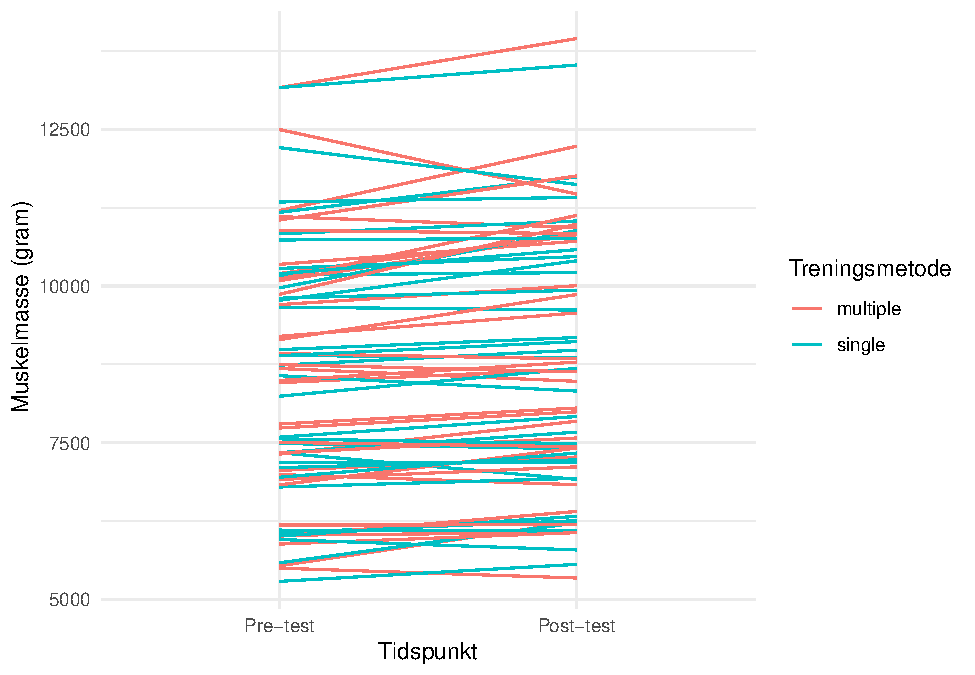
\includegraphics{_main_files/figure-latex/Figur-1.pdf}
\caption{\label{fig:Figur}Figurtekst legg til\ldots{}}
\end{figure}

\hypertarget{diskusjon}{%
\section{Diskusjon}\label{diskusjon}}

Ettersom testing av maksimalt oksygenopptak er en test som gjennomføres til utmattelse, vil man kunne forvente en viss variasjon i testresultatene ettersom opplevd anstrengelse kan påvirkes av flere ulike variabler \citep{halperin2015}. For å redusere konfundering vil flere faktorer være nyttig å ta hensyn til under slik testing. Som nevnt i metoden vil standardisering av matinntak, koffeininntak, utstyr og tidspunkt for gjennomføring av test være med på å kunne sikre intern validitet i resultatene. Eksempler er deltakernes kjennskap til testen, verbal oppmuntring og personer tilstede under testen er andre faktorer som potensielt kan bidra til konfundering. Felles for alle faktorer er at graden av påvirkning på resultatene muligens reduseres ved hjelp av en standardisert testprotokoll. Deltakerne - og testlederne, sin kjennskap til testen er en annen faktor som trolig påvirker resultatene i vårt prosjekt. I dette tilfellet fantes det enkelte deltakere som hadde gjennomført en liknende test flere ganger, og en kan da forvente en mindre grad av variasjon mellom resultatene på pre og post test, sammenlignet med de deltakerne som gjennomførte testen for første gang på pretest. Dette fordi kjennskapen og kunnskapen de tilegnet seg på pre-test, trolig spiller inn på testresultatene. Standardfeilen på 4.04\% kan også tyde på at enkelte av disse resultatene kan være utsatt for konfundering av ulik sort \citep{hopkins2000}.

Grunnen til at vi snakker om standardfeil er at når vi ønsker å måle påvirkningen av trening på en gruppe individer er det viktig å kunne si noe om hva som er endring og hva som er støy (målefeil). Desto mindre støy en test innebærer jo bedre er målingen. Målet som brukes er standardfeil. Hva som danner denne variasjonen som representeres ved typical error er multifaktorelt, men hoveddelen er som oftest biologisk \citep{hopkins2000}.

For å måle standardfeil har vi brukt within subject deviation metoden. Denne metoden påvirkes ikke av at gjennomsnittet endrer seg fra test til test \citep{hopkins2000}. Data for målinger i VO2max fra fem sertifiserte Australske laboratorier fastslo ett gjennomsnitt på 2.2\% for standardfeil \citep{halperin2015}. Data fra det Australske institutt for sport har også fastslått at en standardfeil på omtrent 2\% er riktig for både maksimal og submaksimal O2 \citep{clark2007, robertson2010, saunders2009}. Dette indikerer at med godt kalibrert utstyr og med utøvere som er godt vant med testingen vil en standardfeil på 2\% for det biologiske, og analytiske være riktig \citep{halperin2015}. Vår standardfeil på 4.04\% kan derfor tenkes å være et bilde hvordan det kan se ut med få deltakere, med ulikt utgangspunkt, men også uten skikkelig standardisering av treningshverdagen i forkant av testene. Det kan også tenkes at med et varierende nivå hos deltagerne kan enkelte oppleve en treningseffekt av test 1. Samtidig som andre kanskje ble slitne av å få en test inn i treningshverdagen.

\hypertarget{hello-bookdown}{%
\chapter{Hello bookdown}\label{hello-bookdown}}

All chapters start with a first-level heading followed by your chapter title, like the line above. There should be only one first-level heading (\texttt{\#}) per .Rmd file.

\hypertarget{a-section}{%
\section{A section}\label{a-section}}

All chapter sections start with a second-level (\texttt{\#\#}) or higher heading followed by your section title, like the sections above and below here. You can have as many as you want within a chapter.

\hypertarget{an-unnumbered-section}{%
\subsection*{An unnumbered section}\label{an-unnumbered-section}}
\addcontentsline{toc}{subsection}{An unnumbered section}

Chapters and sections are numbered by default. To un-number a heading, add a \texttt{\{.unnumbered\}} or the shorter \texttt{\{-\}} at the end of the heading, like in this section.

\hypertarget{vitenskapsteori}{%
\chapter{Vitenskapsteori}\label{vitenskapsteori}}

\hypertarget{falsifikasjonisme}{%
\section{1. Falsifikasjonisme}\label{falsifikasjonisme}}

\emph{Hva er Poppers falsifiserbarhetskriterium og hvilket spørsmål skal
dette kriterium gi svar på? Hvorfor mener andre vitenskapsfilosofer
(f.eks. Okasha) at vi ikke trenger å svare på dette spørsmålet? Hvem
synes dere har rett?}

Når man skal diskutere falsifikasjon, er det flere spørsmål som er
aktuelle, hva er vitenskap? er alt som blir publisert vitenskap, og hvor
går i så fall skillet mellom vitenskap og «ikke-vitenskap»? Sistnevnte
er kjent som demarkasjonsproblemet.

Spørsmålene som jeg stiller over, er spørsmål som har vært diskutert av
vitenskapsfilosofer lenge og spesielt de siste hundre årene
\citep{okasha2016} . Karl Raimond Popper har hatt og har stor innflytelse i
disse spørsmålene etter at han kom med sin teori om
falsifikasjonskriteriet \citep{okasha2016} . Denne teorien sier at en
vitenskapelig teori må kunne være mulig å falsifisere (motbevise)
\citep{popper2002}. Dermed kommer Popper med en løsning på
Demarkasjonsproblemet, vitenskap er teorier som teoretisk sett skal være
mulig å motbevise \citep{popper2002}. En teori som ikke kan motbevises er da
ikke-vitenskap, eller som Popper ville sagt, pseudovitenskap
\citep{popper2002}. Popper løfter fram Astrologi som et eksempel på
pseudovitenskap, da det ikke er mulig å falsifisere \citep{popper2002}.
Astrologer baserer seg på empiriske observasjoner og danner horoskoper
med vage teorier sånn at de kan bortforklare et hvert angrep mot læren
\citep{popper2002}. Dette blir på mange måter det motsatte av det Popper
ønsker \citep{popper2002}. En forsker skal heller sette seg teorier for å så
ha som mål å falsifisere de, på denne måten vil man sikre god vitenskap
\citep{popper2002}. Når man prøver å falsifisere en teori vil det være
gjennom deduksjon, teorien har et premiss som empirisk blir testet og
man får svaret sant eller usant. Utfallet blir da enten at teorien blir
falsifisert og da lagt fram som motbevist eller at teorien blir stående.
Ifølge Popper kan ikke teorier bevises, og da er argumentasjon basert på
induksjon heller aldri et alternativ \citep{okasha2016}. Samtidig mener
Popper at teorier som har blitt testet på riktige måter og som ikke har
blitt falsifisert, kan bli «corroborated», altså nesten bevist
\citep{popper2002}. Poppers tanker om disse teoriene som flere ganer ikke er
blitt falsifisert ligner da veldig på en induktiv bekreftelse av en
teori, altså når en teori som mest sannsynlig er sann, men ifølge Popper
er det ikke det samme \citep{okasha2016, popper2002}.

Problemet med Poppers teori om vitenskap kommer tydelig fram når han
ikke kan bekrefte vitenskapelige teorier. Samir Okasha får dette fram i
sin bok om vitenskapsfilosofi \citep{okasha2016}. Okasha løfter fram et
eksempel om personer med Downs Syndrom: Genforskere har funnet ut at
alle som har Down Syndrom har tre kopier av kromosomnummer 21 istedenfor
to \citep[s. 18]{okasha2016}. Genforskere har da basert på et stort utvalg
med personer som har Down Syndrom gjort en konklusjon som gjelder alle
med Down Syndrom \citep{okasha2016}. Dette er da en induktivt bekreftet teori
som er godt dokumentert og som gjør at man kan bygge videre kunnskap
basert på teorien. Popper kunne ikke gjort dette da det ikke er mulig å
gjøre så sterke påstander \citep{okasha2016}. På bakgrunn av dette skulle man
ikke trenger å svare på demarkasjonsproblemet og heller skille mellom
styrket og mindre styrket teorier. Okasha mener at en forskeres rolle
ikke bare handler om å finne ut om en teori er usann, men også å finne
hvilke teorier som er sanne eller mest sannsynlig sanne, og da trenger
man induksjon \citep[s. 19--20]{okasha2016}

\hypertarget{hd-metoden-og-abduksjonbayesisme}{%
\section{2. HD-metoden og abduksjon/Bayesisme}\label{hd-metoden-og-abduksjonbayesisme}}

\emph{Hva er strukturen på et bekreftende vitenskapelig argument ifølge den
hypotetisk deduktive metode? Forklar ut fra Hempels artikkel, men bruk
egne eksempel. Sammenlign også Hempels HD-metode med hvordan
vitenskapelig bekreftelse fungerer ifølge enten abduksjon eller
Bayesianisme}.

I oppgave 1 så jeg på hva en vitenskapelig teori er, nå skal jeg se på
hvordan teorier kan testes. Carl Gustav Hempel mente at det ikke fantes
noen god metode teorier kunne testes og var uenig med Popper
\citep{hempel1966}. Hempel mente at man trengte induktiv argumentasjon i
vitenskapene \citep{hempel1966}. Derfor løftet Hempel fram en metode kaldt
hypotetisk deduktiv metode (HD-metoden), som et bedre alternativ
\citep{hempel1966}. Denne metoden sier ikke noe om hvordan teorier kommer
fram, men den har klare retningslinjer på hvordan man skal teste en
teori og gi den styrke \citep{hempel1966}.

For å forklare HD-metoden bruker jeg følgende eksempel som teori:
Høyintensitets intervalltrening på løp øker det maksimale
oksygenopptaket (VO\textsubscript{2maks}). Ifølge HD-metoden skal man etter at en har
utarbeidet en teori tenke ut empiriske konsekvenser til teorien
\citep{hempel1966}. I vårt tilfelle er det da å finne hvilke empiriske
konsekvenser det er av å få et høyrere VO\textsubscript{2maks}. Man skulle tro at
empiriske konsekvenser av høyere VO\textsubscript{2maks} er et høyere blodvolum og
bedre prestasjon på 5min løpstest. Neste steg er å teste om de empiriske
konsekvensene er sanne, dette skjer gjennom deduktiv testing
\citep{hempel1966}. Dette betyr at økt blodvolum og bedre prestasjon på 5min
løpstest blir satt som premiss for at teorien. Om blodvolumet da har økt
og prestasjonen på 5min løpstest har blitt bedre, gir det en styrke til
teorien om at høyintensiv intervalltrening gir høyere VO\textsubscript{2maks}. I
vanlig deduktiv argumentasjon vil et rett premiss bety at teorien er
sann, men i HD-metoden vil teorien bare bli en grad av induktivt
bekreftet \citep{hempel1966}. HD-metoden vil aldri si at en teori er
bekreftet, da det ikke er mulig å vite om alle argument som kan
forklarer teorien \citep{hempel1966}. Man kan også tenke seg at det er
observasjoner eller resultat som kommer i fremtiden og som motsier det
en har trodd før \citep{hempel1966}. I vårt eksempel kan en se for seg at
høyintensitets intervalltrening under noen forhold ikke gir høyere
blodvolum eller bedre prestasjon på 5min løpstest. HD-metoden er alltid
åpen for at det er andre forklaringer og sier derfor bare noe om en
teoris styrke eller svakhet ut fra det man har testet empirisk
\citep{hempel1966}.

Problemet med HD-metoden er at den empiriske testingen som er bundet til
teorien. Det vil si at man ikke kan endre teorien, selv om resultatet av
en test ender opp med å passe bedre til en annen teori. Charles Sanders
Peirce sin teori kan være løsningen på dette problemet, ved å innføre
abduksjon i tillegg til induksjon og deduksjon \citep{peirce1992}. Abduksjon
handler om at man setter flere teorier, for å deretter forklarer
teoriene og teste de deduktivt (som i HD-metoden) \citep{peirce1992}.
Resultatet fra testene vil da fortelle oss hvilken teori som er sann,
basert på hvilken teori som kan forklarer svarene på testene best
\citep{peirce1992}. En teori som forklarer mest mulig vil være å foretrekke
da man i abduksjon ønsker å ha en teori som er bedre enn andre
tilgjengelig teorier \citep{peirce1992}. Abduksjon blir derav også kaldt
«slutning til den beste forklaringen» fordi en teori skal gi den beste
mulige forklaringen på et fenomen \citep{peirce1992}.

På mange måter ligner HD-metoden og abduksjon på hverandre og begge vil
gå under kvalifisert gjetning \citep{persson2019} . Det som i hovedsak
skiller abduksjon fra HD-metoden er fleksibiliteten og den praktiske
tilnærmingen da det er flere teorier å velge mellom \citep{peirce1992}.

\hypertarget{replikasjonskrisen}{%
\section{3. Replikasjonskrisen}\label{replikasjonskrisen}}

\emph{Hva mener Alexander Bird er forklaringen til at mange resultat i noen
vitenskaper ikke repliseres? Oppsummere Birds argument for dette.
Sammenlign også Birds forklaring med noen av de andre forklaringene som
Bird diskuterer i seksjon 4. Har Bird rett i at hans forklaring er
bedre?}

De siste 20 årene har det blitt identifisert en replikasjonskrise i
vitenskapen \citep{begley2012, ioannidis2005, opensciencecollaboration2015}. Dette handler om at mange studier som
blir gjort på nytt ikke klarer å få det samme resultatet som første
gangen det ble gjort. Det gir oss et stort problem, for hvordan kan man
da stole på vitenskapen? Undersøkelser viser at tillitten til
vitenskapen har falt i England og USA \citep{funk2016}. Dette er også noe
flertallet av forskere anerkjenner som en krise basert på en
spørreundersøkelse gjort på 1500 forskere \citep{baker2016}. Alexander Bird
mener å ha en forklaring til denne replikasjonskrisen \citep{bird2020}.

Bird mener at feilen ligger i en neglisjering av basefrekvens
\citep{bird2020}. Vitenskapen konkluderer rett og slett alt for fort uten å
ta hensyn til basefrekvens \citep{bird2020}. Sånn som vitenskapen er i dag er
det typisk gjort en randomisert kontrollert undersøkelse (RTC) og
resultatet er enten signifikant eller usignifikant basert på P-verdien
\citep{bird2020}. Denne signifikantgrensen som ofte blir satt til 0,05 (5\%)
har da blitt en slags pekepinn på om noe er sant eller usant basert på
om resultatet er over eller under grensen \citep{bird2020}. P-verdien sier
noe om sannsynligheten for at resultatet er falskt positivt
(type-I-feil) \citep{bird2020}. Om P-verdien er 0,05 er det en 5\% sjanse for
at resultatet er falskt positiv \citep{bird2020}. Problemet med dette er at
P-verdien man får etter et forskningsprosjekt bare sier noe om utvalget
som er sett på i den gitte situasjonen \citep{bird2020}. Ved å bruke
basefrekvens vil man se på resultatet basert på populasjonen og hvor
sannsynlig det egentlig er for at resultatet er sant \citep{bird2020}. Et
eksempel på dette, som \citet{bird2020} tar fram, er sannsynligheten for at en
tilfeldig har en sjelden sykdom om vedkommende tester positivt på en
test. Sykdommen hadde en forekomst på 1 til 1000 og testen hadde en
pålitelighet på 95\% \citep{bird2020}. Det er lett å tenke at samsynligheten
er 95\%, men i realiteten er den 2\% \citep{bird2020}. Dette kommer av at man
må regne inn forekomsten i regnestykke gjennom Bayes teorem \citep{bird2020}.
På samme som at det er lett å trekke konklusjonen om at personen i
eksempelet var syk, kan vi dra konklusjoner om at vitenskapelige
hypoteser er sanne \citep{bird2020}. Dette gjør at mange studier faktisk ikke
gir et rett svar, og da ikke er repliserbare \citep{bird2020}.

Andre forklaringer som Bird trekker fram er den statistiske styrken, som
i mange tilfeller ikke er høy nok \citep{bird2020}. Styrken blir i stor grad
styrt av forskningens størrelse (antall deltagere) og gir en
sannsynlighet for å ikke få et falskt negativt resultat (type-II-feil)
\citep{bird2020}. Men Bird mener at dette ikke er en god forklaring fordi en
høy statistisk styrke egentlig fortsatt gir relativt høy sannsynlighet
for å få en type-II-feil \citep{bird2020}. Bird viser til en utregning hvor
det er høyere statistisk styrke enn i «vanlig» vitenskap, men at det
fortsatt er 31\% sjanse for å få type-II-feil \citep[s. 12-14]{bird2020}. Det
vil være bra for vitenskapen å få opp den statistiske styrken, men kan
ikke forklarer krisen som vitenskapen står i \citep{bird2020}.

Juks og dårlig praksis i vitenskapen vil kunne forklare noe av
replikasjonskrisen, men det er vanskelig å sette en konklusjon basert på
det man har sett av studier så langt \citep{bird2020}. Det er derfor ikke
gode nok holdepunkt til å mene at det er dårlig moral rundt vitenskapen
som er hele forklaringen på krisen \citep{bird2020}.

Basert på det \citet{bird2020} skriver, er det tydelig at det er hans egen
forklaring som gir mest styrke til teorien om at vitenskapen er i en
krise. Det er tydelig at folk som driver vitenskap trenger en større
forståelse av statistikk og sannsynlighet \citep{bird2020}. Gjennom et større
hensyn til basefrekvensen vil man utarbeide bedre teorier og være mer
forsiktig med å si at noe er gjeldene for en hel populasjon \citep{bird2020}.

\hypertarget{studiedesign}{%
\chapter{Studiedesign}\label{studiedesign}}

\hypertarget{introduksjon-1}{%
\section{Introduksjon}\label{introduksjon-1}}

Mennesker i vesten lever lenger og lenger, og eldrebølgen er et faktum, derfor er det et stort behov for å finne ut hvordan eldre mennesker kan bevare helsen best mulig. I denne rapporten skal jeg se på fem studier som har sett på styrketrening som en metode for å bedre helsen til eldre mennesker \citep{geirsdottir2012, schott2019, turpela2017, vikberg2019, vincent2002}. Alle fem studiene ønsker å finne ut hvordan man kan legge opp styrketrening som gir effektiv og god effekt på helsen (mentalt og fysisk) og dermed gjøre det lettere å gi gode treningsanbefalinger. En oppsummering av studiene er vist i tabell 1.

I fire av studiene ble det sett på forskjellige måter man rent praktisk bør gjennomføre styrketrening \citetext{\citealp[ ]{schott2019}; \citealp{turpela2017}; \citealp{vikberg2019}; \citealp{vincent2002}}. I \citet{schott2019} ble det for eksempel sett på responsen det var av å trene med styrketreningsapparater mot frivektstrening \citep{schott2019}. Studien til \citet{geirsdottir2012} skiller seg fra de andre da den hovedsakelig så på den generelle effekten av trening \citep{geirsdottir2012}. Den så som de andre på styrke- og muskeladaptasjoner, men inkluderte et spørreskjema om hvordan treningen påvirket livskvaliteten \citep{geirsdottir2012}.

På bakgrunn av studiespørsmålene og svarene de vil gi oss, vil studiene gi en styrke til den allerede etablerte anbefalingen om at eldre bør trene styrke for å opprettholde eller bedre helsen \citep[ \citet{vincent2002}]{geirsdottir2012, schott2019, turpela2017, vikberg2019}. I tillegg vil studiene gjøre det lettere å gi gode anbefalinger da de løser noen praktiske spørsmål rundt selve gjennomføringen av styrketrening \citetext{\citealp[ ]{geirsdottir2012}; \citealp{schott2019}; \citealp{turpela2017}; \citealp{vikberg2019}; \citealp{vincent2002}}. \citet{vikberg2019} foreslår at en enkel form for styrketrening som man kan gjøre hjemme er nok for å styrke muskulatur og bedre helsen. Dette vil gjøre styrketreningseffekten oppnåelig for alle, og ikke bare de som trener på treningssenter \citep{vikberg2019}.

\hypertarget{metode-1}{%
\section{Metode}\label{metode-1}}

Fire av studiene var RTC-studier hvor det var en, to eller tre intervensjonsgrupper og en kontrollgruppe \citep{schott2019, turpela2017, vikberg2019, vincent2002}. Hvem som var i hvilke grupper, ble randomisert tilfeldig. Antallet i gruppene var nesten likt fordelt i intervensjon og kontroll med unntak av \citet{vincent2002} . «Nesten likt» vil si at det stort sett var flere i de gruppene det krevde mest av (treningsgruppene), samtidig var det gruppene med flest frafall, sånn at det ved studieslutt nesten var utlignet \citep{schott2019, turpela2017, vikberg2019}. I \citet{vincent2002} var det større forskjell på kontroll og intervensjon (16 i kontroll, 24 og 22 i intervensjon) uten at det blir opplyst noen grunn til det. Å ha en blokkrandomisering som de tre andre nevnt over, ville gitt studien et styrket design. Når det er forskjellige størrelser vil det bli vanskeligere å sammenligne, da mindre grupper gir bredere konfidensintervall og lavere statisk styrke \citep[s. 63, 146]{hulley2013}.

Da dette er studier som ser på trening er «blinding» vanskelig, dermed nevnte studiene heller ikke noe om dette \citep{geirsdottir2012, schott2019, turpela2017, vikberg2019, vincent2002}. For å unngå forskingsfusk er det likevel gunstig at testpersonell ikke vet hvem som er i hvilken gruppe, da testpersonell skal gjennomføre alle tester like godt, selv om man ofte ønsker et resultat i favør hypotesen \citep[s. 148-149]{hulley2013}.

\citet{geirsdottir2012} var en klinisk studie uten kontrollgruppe, de hadde altså en stor gruppe (265 kvinner og menn) som trente samme styrketreningsprogrammet. At de ikke hadde kontrollgruppe innrømmet studiegruppen selv at var en svakhet \citep{geirsdottir2012}. Samtidig poengterte de at eldre mennesker ikke kan forvente en økning i styrke, muskelmasse og muskelfunksjon uten å trene og sånn sett mente de at det var nok å sammenligne med testresultat ved start \citep{geirsdottir2012}. Det er mulig å forstå argumentasjonen til \citet{geirsdottir2012} når de i tillegg har såpass mange deltagere som de har. Samtidig hadde en definert kontrollgruppe gjort studien sterkere som en studie som skulle finne ut av noe \citep[s. 87]{hulley2013}. Studien vil gå under kategorien Case-serie som er mer egnet til å se på karakteristika og i denne sammenhengen av styrketrening på eldre \citep[s. 87]{hulley2013}. Noe de også i en viss grad gjorde når resultatet av spørreskjema om livskvalitet var noe av det viktigste \citep{geirsdottir2012}. Denne karakteristikk-egenskapen som studien kunne nok kommet bedre frem.

Populasjonen som er ønsket å treffe er eldre kvinner og menn som var relativt friske \citep{geirsdottir2012, schott2019, turpela2017, vikberg2019, vincent2002}. Ingen av studiene har en eksplisitt definisjon av «eldre», men totalt i studiene var det et aldersspenn på 60-92 og gjennomsnittsalderen i de forskjellige studiene var rundt 70år (flest rett under) \citep{geirsdottir2012, schott2019, turpela2017, vikberg2019, vincent2002}. Den eldre befolkningen er en svært heterogen gruppe, noe som gjør det vanskelig med ekskluderingskriterier. Studiene godtok da det som ble definert som milde sykdommer som ikke påvirker treningen. Unntaket er til en viss grad \citet{vikberg2019} hvor det ikke var andre inklusjonskretierier enn at de ikke måtte ha sarkopeni. Samtidig kan det tyde på at det var relativt god helse blant deltagerene da de alle var 70 år, ikke hadde sarkopeni og klarete å gjennomføre treningen \citep{vikberg2019}. Totalt sett treffer studiene godt på populasjonen da alle har et høyt antall deltagere og har kvalifikasjonskriterier som gjør det mulig for «vanlig» eldre folk å være med \citep{geirsdottir2012, schott2019, turpela2017, vikberg2019, vincent2002}.

Rekruteringen av deltagere ble gjort ved hjelp av brev og annonser med unntak av \citeauthor{schott2019} \citetext{\citeyear{schott2019}; \citealp{geirsdottir2012}; \citealp{turpela2017}; \citealp{vikberg2019}; \citealp{vincent2002}}. Han hentet deltagere fra en treningsgruppe som var etablert på studiestedet \citep{schott2019}. Felles for alle studiene var at det va en frivillig deltagelse \citep{geirsdottir2012, schott2019, turpela2017, vikberg2019, vincent2002}. \citet{schott2019} og \citet{vincent2002} utrykte et krav om at det måtte være statistisk styrke på 80\%. \citet{schott2019} gjorde også et estimat hvor de så at det var behov for 26 deltagere for å se en signifikant forskjell ved signifikantgrense på 5\% når de godtok en sannsynlighet på 80\% (de inkluderte 32 personer). De andre studiene nevnte ikke noe om statistisk styrke, og kunne med fordel vist til en estimering av deltagere som krevdes for en gitt statistisk styrke. \citet{turpela2017} innrømmet også at det kunne bli vanskelig å se forskjell mellom gruppene da utrente ofte får god effekt uansett, noe som kunne blitt kontrollert for om man hadde gjort en powerbergening og inkludert tilstrekkelig deltagere.

Alle fem studiene hadde pre-post-design hvor Scott et al.~også i tillegg hadde tester i uke 10/26 og 6 uker etter post-testen i uke 26 \citep{geirsdottir2012, schott2019, turpela2017, vikberg2019, vincent2002}. I alle studiene ble det gjort idrettsfysiologiskse tester av styrke, men også funksjonelle tester som hadde som mål å se hvordan styrken kom til utrykk i dagligdagse gjøremål (gå test, gripe test osv.) \citep{geirsdottir2012, schott2019, turpela2017, vikberg2019, vincent2002}. \citet{geirsdottir2012} la som nevnt også en del vekt på spørreskjema som ble gitt før og etter intervensjon. \citet{schott2019} hadde også et spørreskjema, men dette ble bare gitt etter og var en evaluering av treningen. Treningen som ble gjennomført av intervensjonsgruppene ble gjort på treningssenter eller treningslokale på studiestedet \citep{geirsdottir2012, schott2019, turpela2017, vikberg2019, vincent2002}. \citet{vincent2002} fikk deltagerne til å sende inn treningsdagbøker for hver økt som det det ble gitt tilbakemelding på. I de fire andre studiene var det trenere eller med kvalifisert kurs eller utdanning som veiledet deltagerne igjennom økten \citep{geirsdottir2012, schott2019, turpela2017, vikberg2019}. Kontrollgruppen ble instruert i å leve som vanlig og ikke trene \citep{schott2019, turpela2017, vikberg2019, vincent2002}. Treningsperiodene var fra 10 uker til 26 uker \citetext{\citealp{geirsdottir2012}; \citealp{schott2019}; \citealp[\href{mailto:2019;@Turpela}{}][]{turpela2017}; \citealp{vikberg2019}; \citealp{vincent2002}}.

Studiene hadde som nevnt som mål å finne ut hvordan eldre bør trene og hvilke effekter det er av styrketrening \citep{geirsdottir2012, schott2019, turpela2017, vikberg2019, vincent2002}. For å finne ut dette ble det sett på forskjellige variabler for styrke, kroppssammensetning (spesielt fettfri masse), muskelstørrelse, men også variabler som skulle reflektere dagligdagse gjøremål \citep{geirsdottir2012, schott2019, turpela2017, vikberg2019, vincent2002}. \citet{vincent2002} la for eksempel en del vekt på en trappetes hvor deltagerne skulle gå en trapp så fort som mulig. Dette er viktig da noe av hovedgrunnen for å trene styrke for eldre nettopp er å mestre dagligdagse gjøre mål \citep{vincent2002}.

I analysen av studiene var det ønskelig å finne forskjeller i resultat mellom grupper, her ble det brukt forskjellige statistiske tester. I tre av studiene hvor det var en eller to grupper ble brukt paret t-test får så se forskjell innad i gruppene \citep{geirsdottir2012, vikberg2019, vincent2002}. \citet{vincent2002} brukte ANCOVA for å se forskjell innad i gruppe og la da også inn effekten av tid. Verdiene ved studiestart ble satt som en kovariat og satt opp mot post-resultatet per person for å se forskjell fra pre til post \citep{vincent2002}. \citet{turpela2017} brukte her en-veis-ANOVA for kontrollere for ulikheter ved pre-test. For å se på forandring i gruppene ble det brukt uavhengig t-test og ANCOVA hvor man også kunne se på effekten av tid og enveis gjentatte målinger \citep{schott2019, turpela2017, vikberg2019, vincent2002}. \citet{schott2019} brukte også MANCOVA for å gjøre statistikk på variablene som ble mål flere enn 2 ganger og på spørreskjammaet han brukte. \citet{geirsdottir2012} brukte Wilconxon's test for analyse av spørreskjemaet sitt. Tre av studiene brukte også post hoc tester som vil gi et mer troverdig resultat da den kontrollerer resultatet for falsk positiv \citep[s. 50-52]{hulley2013}. \citep{schott2019, turpela2017, vincent2002}. Alle hadde signifikantgrense ved P = 5\% med unntak av en ANCOVA-test \citet{vikberg2019} gjorde som gjorde en interaksjon mellom kjønn og intervensjon, hvor P = 10\% \citep{geirsdottir2012, schott2019, turpela2017, vincent2002}. Denne interaksjonen til \citet{vikberg2019} vil med dette lettere godta at det er en forskjell mellom kjønn.

\hypertarget{resultat}{%
\section{Resultat}\label{resultat}}

Tre av studeiene studiene, som sammenlignet intervensjon mot kontroll, ble det ikke sett forskjell på muskelmasse, men \citet{vikberg2019} fant forskjell i muskelmasse \citep{schott2019, turpela2017, vincent2002}. \citet{vikberg2019} fant ikke forskjell i styrke fra kontrollgruppen, men de gjorde de tre andre \citep{schott2019, turpela2017, vincent2002}. På funksjonell styrke gav alle studiene positiv effekt på funksjonelle tester \citep{geirsdottir2012, schott2019, turpela2017, vikberg2019, vincent2002}. I de studiene som sammenlignet flere treningsprotokoller var det liten forskjell mellom det forskjellige treningsprotokollene, men alle skilte seg fra kontrollgruppen \citep{schott2019, turpela2017, vikberg2019, vincent2002}. \citet{geirsdottir2012} fant en liten forbedring av livskvalitet. Alt i alt greide de delvis å gi et positivt svar på hypotesen \citep{geirsdottir2012, schott2019, turpela2017, vikberg2019, vincent2002}.

Alle studiene konkludere med at styrketrening fungerte \citep{geirsdottir2012, schott2019, turpela2017, vikberg2019, vincent2002}. For å oppsummere anbefalingene, er det nok å trene styrke 1-2 gagner i uken, så lenge det er helkroppsøkt \citep{turpela2017, vikberg2019}. En ytterlig effekt vil man få om man trener med frivekter, spesielt på ben og triceps, som er viktige muskelgrupper for eldre \citep{schott2019}. Det er også nok å gjøre 13 rep på 50\% 1RM \citep{vincent2002}. Antall serier er ikke sett på, men basert på studiene burde 1-2 være nok \citep{geirsdottir2012, schott2019, turpela2017}. Det kommer også fram at all trening som ble sett på gav en effekt \citep{geirsdottir2012, schott2019, turpela2017, vikberg2019, vincent2002}. Treningen vil vedlikeholde muskelmassen din, øke styrken din, gjøre praktiske gjøremål lettere og det vil kunne øke livskvaliteten din \citep{geirsdottir2012, schott2019, turpela2017, vikberg2019, vincent2002}. Denne konklusjonen og anbefalingen gjelder for relativet friske eldre mennesker som ikke er vant til å trene og som har en lav muskelmasse, dog ikke kritisk lav \citep{geirsdottir2012, schott2019, turpela2017, vikberg2019, vincent2002}.

\hypertarget{videre-forskning}{%
\section{Videre forskning}\label{videre-forskning}}

Det er enda ikke veldig tydelig hvilke treningsprogram som gir god effekt på bedret funksjonsevne \citep{turpela2017}. \citet{schott2019} foreslår at studeier med frivekter kan være løsningen. I tillegg burde man gjøre studier hvor man kontrollerer proteininntaket hos eldre da dette kan være så lavt at det påvirker styrkefremgangen \citep{turpela2017}.

Tabell 1. Oppsummering av artiklene

\begin{longtable}[]{@{}
  >{\raggedright\arraybackslash}p{(\columnwidth - 12\tabcolsep) * \real{0.01}}
  >{\raggedright\arraybackslash}p{(\columnwidth - 12\tabcolsep) * \real{0.14}}
  >{\raggedright\arraybackslash}p{(\columnwidth - 12\tabcolsep) * \real{0.10}}
  >{\raggedright\arraybackslash}p{(\columnwidth - 12\tabcolsep) * \real{0.06}}
  >{\raggedright\arraybackslash}p{(\columnwidth - 12\tabcolsep) * \real{0.41}}
  >{\raggedright\arraybackslash}p{(\columnwidth - 12\tabcolsep) * \real{0.12}}
  >{\raggedright\arraybackslash}p{(\columnwidth - 12\tabcolsep) * \real{0.16}}@{}}
\toprule
Studie & Studiespørsmål & Hypoteser & Logikk & Metode & Resultat & Interferes \\
\midrule
\endhead
\citet{turpela2017} & Hvordan påvirker treningsfrekvensen muskelstyrke, muskelmasse og funksjonell kapasitet hos utrente eldre mennesker? & Hypotese: To til tre treninger i uken er bedre enn en trening.

Alternativ hypotese: Utrente vil ha god effekt uansett og da gjøre forskjellen på vanskelig å se. & Det vil bli enklere å \textbar{} gi klare råd om hvor ofte eldre bør trene styrke for å oppnå treningseffekt. & 4 grupper basert på antall treninger i uken: ingen økter, 1 økt, 2 økter og 3 økter. Intervensjonsperioden var 6 måneder med 3 måneder tilvenning i forkant. Styrketester og funksjonell kapasitet ble testet før og etter. Treningsøktene var tradisjonell tung og eksplosiv trening. 106 kvinner og menn (64-75 år) som var friske med unntak «normale» alderssjukdommer.

Ble brukt en-veis-ANOVA og en-veis-ANOVA med gjentatte målinger & Ikke sammenheng \textbar{} mellom treningsfrekvens og ganghastighet eller kroppssammensetning. Alle skilte seg fra kontrollgruppen Dose-respons i forhold til 1RM og dynamisk styrke (i treningsapparat) & Sunne eldre vil ha en gunstig effekt av å trene lavfrekvens helkropps styrketrening (1-2 ganger i uken). \\
\citet{schott2019} & Studien hadde to \textbar{} formål:

1.Sammenligne effekten av intensiv frivektstrening med apparattrening hos godt fungerende eldre mennesker.

2.~~~~~~~~~ Se om intensiv trening med frivekter er gjennomførbart på denne gruppen & Begge gruppene vil ha \textbar{} en fremgang i styrke, men gruppen som trener med frivekter vil få et bedre resultat sammenlignet med gruppen som trente med treningsapparat. & Vil gjøre det lettere \textbar{} å gi treingsanbefalinger for godt fungerende eldre & 32 friske kvinner \textbar{} og menn mellom 60 og 86 år ble fordelt i to grupper hvor den ene trente med frivekter, mens den andre trente med apparat.

Det ble gjennomført to treninger i uken hvor øvelsene ble gjort i 3 sett og 10-12 repetisjoner (10RM). Alle økter ble avsluttet med 20 min utholdenhetstrening. Testing av styrke og utholdenhet ble gjort ved start, 10 uker, 26 uker og 6 uker etter intervensjon (uten trening). Det ble også utfylt spørreskjema etter intervensjon. Statistikk ble gjort ved uavhengig t-test, paret t-test, MANCOVA, Cohens d og Pearsons korrelasjon. & Begge gruppene økte i \textbar{} alle øvelser og gjorde det bedre på dynamiske styrketester. For triceps og ben var det større effekt av å trene med frivekter. Frivektstrening var mer motiverende. & Trening både med frivekter og maskin gir god styrkeeffekt, men frivektstrening gir ytterlige effekt på ben og triceps. Disse to muskelgruppene er viktige for å forebygge fall og i dagliglivet, frivektstrening er derfor å anbefale for eldre som er godt fungerende. \\
\citet{vikberg2019} & Effekten av 10-ukers trening med enkle styrkeøvelser og lite utstyr ledet av instruktør på personer med presarkopeni. Hovedspørsmålene er om treningen gir effekt på funksjonell styrke og om det påvirker kroppssammensetningen & Styrketreningen vil \textbar{} gi positiv effekt på funksjonell styrke & Eldre kan på en enkel måte få god effekt av styrketrening. & 70 kvinner og menn med presarkopeni ble fordelt i kontroll (36) og intervensjonsgruppe (34). Intervensjonsgruppen trente tre gruppetreninger i uken i 10 uker. Det var ingen tydelige ekskluderingskriterier. Treningene var helkroppsøkter med enkle øvelser. Intensiteten skulle ligge på RPE mellom 6 og 7 (skala 1-10). Det ble gjort et testbatteri før og etter bestående av funksjonelle tester i tillegg til tester av kroppssammensetning. Paret T-test ble brukt for å se forskjell innad i gruppene. ANCOVA ble brukt få se forskjell mellom gruppene. & Det var økning i styrke fra post til pre hos intervensjonsgruppen, men de skilte seg ikke fra kontroll. Kroppssammensetning var bedret innad i gruppen og i forhold til kontroll. & Styrketrening med enkelt utstyr som man kan gjøre nesten hvor som helst er effektivt for å hindre tap av muskelstyrke og øke muskelmasse for eldre med presarkopeni \\
\citet{geirsdottir2012} & Hva er styrketreningseffekten på eldre mennesker, spesielt med tanke på helse relatert til livskvalitet, men også styrke, kroppssammensetning og funksjonell kapasitet & Styrketreningen vil \textbar{} gi god effekt på muskelmassen og styrken som igjen vil øke helse relatert til livskvalitet. & Styrketrening vil gi \textbar{} høyere livskvalitet hos eldre & 265 friske kvinner og menn mellom 65 og 92 år gikk igjennom et 12 ukers treningsprogram med tre økter i uken med. Øktene var helkroppsprogram (3 sett, 6-8 rep på 75-80\% av 1RM per øvelse). Motstanden ble økt 5-10\% hver uke. Før og etter ble det testet styrke, kroppssammensetning, funksjonell styrke og tatt spørreskjema om livskvalitet. Statistikk mellom de som droppet ut og de andre ble analysert ved uavhengig t-test. Paret t-test ble brukt for å se på forskjell mellom pre og post. Wilcoxon test ble brukt for å se på pre og post spørreskjema. Persons og Spearmans r ble brukt for å se på korrelasjoner mellom spørreskjemavariabler og kroppssammensetning, styrke og funksjon. & Det var en økning i muskelmasse, styrke og funksjonell kapasitet. Det var en liten, men signifikant økning i livskvalitet & 12 uker med styrketrening vil gi god effekt på styrke, kroppssammensetning og muskelmasse. Dette vil igjen gi bedre livskvalitet. Ved styrketrening vil en også hindre fallet i muskelstyrke og muskelmasse. \\
\citet{vincent2002} & Er det forskjell på treningseffekten av å trene høyere vekt og lavere antall repetisjoner og lavere vekt og flere repetisjoner hos eldre mennesker & Styrketrening med lavere vekt og flere repetisjoner fungerer like bra som høy vekt og få repetisjoner. & Man kan anbefale trening som oppleves lettere og som er mindre skadeutsatt. & 62 Friske kvinner og \textbar{} menn mellom 60 og 83 år trenete eller var i kontroll i 26 uker. De som trente, trente enten 50\% av 1RM *13 rep eller 80\% av 1RM 8 rep i en serie per treningsapparat (volum blir ca. det samme for begge). Basert på borgs skala (6-20), ble det gjort økninger i vekt på treningen. Før og etter perioden ble det testet kroppssammensetning, diet, styrke, utholdende styrke og trappetest. ANOVA ble brukt for å se forskjell innad og mellom gruppene over tid. For de endelige resultatet ble ANCOVA brukt for å se på forskjeller & Begge \textbar{} treningsgruppene fikk økning i muskelstyrke og muskelutholdenhet, samt i trappetesten i forhold til kontroll, men ingen forskjell mellom \textbar{} treningsgruppene. & Eldre friske mennesker kan få like godt resultat med 13 rep på 50\% av 1 RM, 8 rep på 80\% av 1RM. Dette gjør styrketrening enklere i tillegg til lavere skaderisiko. \\
\bottomrule
\end{longtable}

\hypertarget{vs-3-sett}{%
\chapter{1 vs 3 sett}\label{vs-3-sett}}

\hypertarget{introduksjon-2}{%
\section{Introduksjon}\label{introduksjon-2}}

Styrketrening blir mer og mer populært i det norske samfunn, og tall fra Levekårundersøkelsen i 2019 viser at 4 av 5 trener styrke en gang i uken \citep{statistisksentralbyrå2019}. Konseptet styrketrening handler om at man ønsker å styrke kroppen, men hvordan gjør man det på lettests mulig måte og med best mulig effekt? Tradisjonelt gjør man en styrkeøvelse X antall ganger (repetisjoner) og i X antall serier (sett). Men hvor mye har det å si at man gjør ett eller flere sett? Flere studier har sett på effekten av å gjøre ett sett og tre sett \citep{galvão2005, hass2000, krieger2009, radaelli2014, schoenfeld2019}. Resultatet i studiene er sprikende. Noen studier finner ikke forskjell mellom grupper som trener ett og tre sett \citetext{\citealp[ ]{hass2000}; \citealp{radaelli2014}}, mens andre studier ser at begge gruppene øker, men tre sett gir en ytterlige effekt på styrke \citep{krieger2009, galvão2005}. Det er også sett at man kan oppnå like styrkeeffekter, men at økningen av muskelmasse trenger større volum enn ett sett for å gi effekt \citep{schoenfeld2019}.

Basert på statistikken fra \citet{statistisksentralbyrå2019} er det mange som får til å trene styrke en gang i uken, men vi vet at skal må få gunstig styrkeeffekt, må man trene to til tre ganger i uken \citep{schoenfeld2016}. På bagrunn av dette vil det være gunstig å finne ut av spørsmålet om ett sett er nok, da en treningsøkt tar mye kortere tid. Noe av det som gjør at det er vanskelig å dra en tydelig konklusjon av studiene på området er at det vil være individuelle variasjoner. Derfor er det interessant å gjøre en studie hvor man trener ett sett på ene benet og tre sett på det andre benet. På denne måten vil en sikre at framgangen ikke blir forskjellig på bakgrunn av gruppeforskjeller.

I denne studien ønsker vi å se videre på effekten av ett og tre sett, hvor vi først ønsker å se på effekten av en kort treningsperiode (fem uker) og en lengre treningsperiode (12 uker). Vi hypotetiserer at begge gruppene vil ha en god framgang i både styrke og muskelstørrelse, men at gruppen som trener tre sett vil få en bedre styrkefremgang ved både fem og 12 uker.

\hypertarget{metode-2}{%
\section{Metode}\label{metode-2}}

\hypertarget{etikk}{%
\subsection{Etikk}\label{etikk}}

Alle deltagere i studien ble informert om potensielle risikoer ved trening og testing og eventuelle ubehagelige og anstrengende situasjoner og gav et informert samtykke. Alle prosedyrer er i tråd med Helsinkideklarasjonen.

\hypertarget{deltagere}{%
\subsection{Deltagere}\label{deltagere}}

Det ble rekruttert 41 kvinner og menn til en treningsperiode på 12 uker. Kriterier for å være med var at de måtte være mellom 18-40 år og ikke røyke. De måtte også være vant til å trene (mer enn en økt uka det siste året). ~I analysene av styrkefremgang ble bare 29 deltagere inkludert de resterende ikke møtte opp på test ved fem uker. 34 deltagere ble analysert for muskelmasseøkning (bare test ved pre og post), resterende gjennomførte ikke studien (fem stk pga. smerter, en stk. pga skade som ikke hadde med studien å gjøre og en pga. ikke fulgte protokoll).

\hypertarget{trening}{%
\subsection{Trening}\label{trening}}

Trenging som ble gjennomført var et helkroppstreningsprogram hvor treningen av ble gjort forskjellig på høyre og venstre fot. De ene bene trente ett sett, mens det andre trente tre sett. Hvilket ben som trente hva, ble randomisert. Antall repetisjoner 0-2 uker var 10 repetisjoner maksimum (RM), uke 2-5 var det 8RM, uke 5-12 var det 7RM. Det ble gjort treninger i uken, med unntak av ukene hvor det ble gjort test. Alle økter ble gjort på ved kvalifiserte trenere (91\% av øktene, resterende økter ble gjort uten trener for at det skulle bli gjennomførbart). Øvelsene på bena ble gjort i denne rekkefølgen: unilateral benpress, knefleksjon og knefleksjon med enten ett sett eller tre sett. Det ene settet ble gjort mellom andre og tredje sett i tre sett serien. Etter bedøvelsene ble to sett av øvelser på overkroppen gjort I to sett: bilateral benkpress, nedtrekk og enten skulderpress eller sittende roing (gjort annenhver økt).~ Pauser mellom sett var 90-180 sekund og pause mellom økten var på minimum 24 timer.

\hypertarget{testing}{%
\subsection{Testing}\label{testing}}

\hypertarget{styrketester}{%
\subsubsection{Styrketester}\label{styrketester}}

Styrketestne ble gjort ved pre, etter fem uker og ved post (12 uker). Tre av testene ble gjort som unilateral kneekstensjon i dynamometer (Cybex 6000, Cybex International, Medway USA). I forkant av testingen ble en standardisert oppvarming gjennomført på ergometersykkel i 5 minutter. Dynamometeret ble justert av testleder sånn at individuelle innstillinger ble gjort. Før hver test ble det gjort standardiserte oppvarmingsrepetisjoner i dynamometeret. Isokinetisk (isok) og isometrisk (isom) styrke ble målt ved maksimalt dreiemoment målt i newtonmeter, og ble notert for hver test (isok120, isok240 og isok60 grader per sekund bevegelseshastighet og isom0 (kneet i 60 graders vinkel)). Det ble gitt to forsøk ved isok60 og isom60 og tre forsøk ved isok240 og isok120 og høyeste ble registrert.

De to andre testene var 1RM-tester i unilateral kneekstensjon og benpress. Som oppvarming ble det gjort 10, 6 og 3 repetisjoner ved henholdsvis 50, 75 og 85\% av forventet 1RM. Deretter ble 1RM funnet ved at vekten ble økt gradvis til de de ikke klarte å fullføre full bevegelse i øvelsen. Den høyeste gjennomførte repetisjonen ble satt som 1RM.

Resultatet ble regnet om til en kombinert score som er et gjennomsnitt av alle styrketestene.

\hypertarget{testing-av-muskelmasse}{%
\subsubsection{Testing av Muskelmasse}\label{testing-av-muskelmasse}}

Ved pre og post-test ble det brukt «dual-energy X-ray absorptiometry» (DXA). Deltagerne fikk beskjed om å faste de to timene før test og å unngå fysisk aktivitet 48 timer før. ~

\hypertarget{statestikk}{%
\subsection{Statestikk}\label{statestikk}}

For å se forskjell mellom 1 sett og 3 sett ble ANCOVA brukt, hvor det ble tatt hensyn til at dataene er korrelerte. Dette er da man gjør to forskjellige protokoller på samme person. Det ble også sett på forskjeller innad i kjønn. For muskelmasse ble det sett på forskjell på fra pre til post. Endring i muskelmasse ble analysert ved pre til 5 uker, 5 uker til post, og pre til post. En P-verdi under 0,05 blir sett på som signifikant endring. Alle tall er gitt som gjennomsnitt med standardavvik. Tabeller, figurer og analyser ble gjort i RStudio (versjon 1.4.1717; R Founadtion for Statistics Computing, Vienna AT).

\hypertarget{resultat-1}{%
\section{Resultat}\label{resultat-1}}

\hypertarget{muskelmasse}{%
\subsection{Muskelmasse}\label{muskelmasse}}

Benet som trente tre sett økte signifikant mer enn benet som trente ett sett, med henholdsvis økning på 3.37\% (±4.59\%) og 2.05\% (±3.62) (p \textless{} 0.05) (figur 1). Det var ingen forskjell mellom benene ved pre.

\begin{Shaded}
\begin{Highlighting}[]
\NormalTok{knitr}\SpecialCharTok{::}\NormalTok{opts\_chunk}\SpecialCharTok{$}\FunctionTok{set}\NormalTok{(}\AttributeTok{echo =} \ConstantTok{TRUE}\NormalTok{)}
\FunctionTok{options}\NormalTok{(}\AttributeTok{knitr.duplicate.label =} \StringTok{"allow"}\NormalTok{)}

\NormalTok{figurmuskel}
\end{Highlighting}
\end{Shaded}

\begin{figure}
\centering
\includegraphics{_main_files/figure-latex/figur-1.pdf}
\caption{\label{fig:figur}Figur 1 viser økningen i muskelvekst fra pre-test til post-tesst for alle forsøkspersoner skildt ved single- sett (1 sett) og multiple- sett (3 sett).}
\end{figure}

\hypertarget{muskelstyrke}{%
\subsection{Muskelstyrke}\label{muskelstyrke}}

Begge gruppene økte i styrke fra pre til uke 5 og uke 5 til post (figur2) (p \textless{} 0.05). Den største økningen kom for begge treningsmetodene mellom pre og uke fem (begge p \textless{} 0.01) (tabell 1). Fra uke 5 og post var det en økning på 10\% for benet som trente 3 sett og 6.8\% for benet som trente 1 sett (begge p \textless{} 0.01). Benet som trente tre sett økte mer en benet som trente ett sett ved både 5 uker og ved post-test (tabell 1).

\begin{Shaded}
\begin{Highlighting}[]
\FunctionTok{options}\NormalTok{(}\AttributeTok{knitr.duplicate.label =} \StringTok{"allow"}\NormalTok{)}
\NormalTok{figurstyrke}
\end{Highlighting}
\end{Shaded}

\begin{figure}
\centering
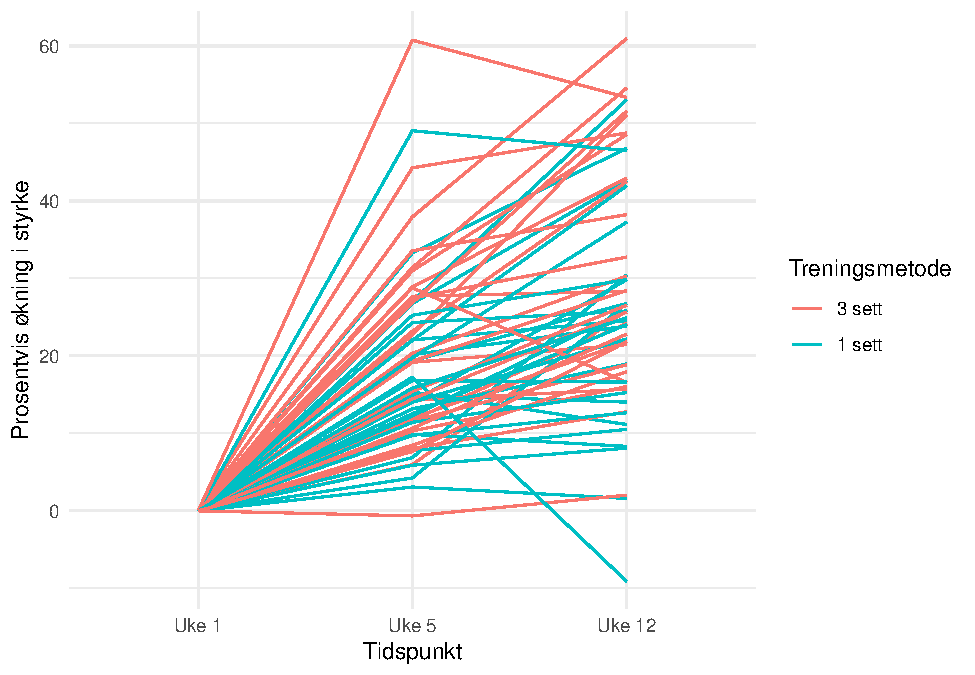
\includegraphics{_main_files/figure-latex/styrkefigur-1.pdf}
\caption{\label{fig:styrkefigur}Figur 2 viser økningen i muskelstyrke, fra pre-tests til 5 uker og 5 uker til post-test for alle forsøkspersoner skildt ved single- sett (1 sett) og multiple- sett (3 sett).}
\end{figure}

\begin{Shaded}
\begin{Highlighting}[]
\FunctionTok{options}\NormalTok{(}\AttributeTok{knitr.duplicate.label =} \StringTok{"allow"}\NormalTok{)}
\NormalTok{tabellstyrke}
\end{Highlighting}
\end{Shaded}

\providecommand{\docline}[3]{\noalign{\global\setlength{\arrayrulewidth}{#1}}\arrayrulecolor[HTML]{#2}\cline{#3}}

\setlength{\tabcolsep}{2pt}

\renewcommand*{\arraystretch}{1.5}

\begin{longtable}[c]{|p{0.75in}|p{0.98in}|p{0.98in}}



\hhline{>{\arrayrulecolor[HTML]{666666}\global\arrayrulewidth=2pt}->{\arrayrulecolor[HTML]{666666}\global\arrayrulewidth=2pt}->{\arrayrulecolor[HTML]{666666}\global\arrayrulewidth=2pt}-}

\multicolumn{1}{!{\color[HTML]{000000}\vrule width 0pt}>{\raggedright}p{\dimexpr 0.75in+0\tabcolsep+0\arrayrulewidth}}{\fontsize{11}{11}\selectfont{\textcolor[HTML]{000000}{\global\setmainfont{Arial}{\ }}}} & \multicolumn{1}{!{\color[HTML]{000000}\vrule width 0pt}>{\raggedright}p{\dimexpr 0.98in+0\tabcolsep+0\arrayrulewidth}}{\fontsize{11}{11}\selectfont{\textcolor[HTML]{000000}{\global\setmainfont{Arial}{Uke\ 5}}}} & \multicolumn{1}{!{\color[HTML]{000000}\vrule width 0pt}>{\raggedright}p{\dimexpr 0.98in+0\tabcolsep+0\arrayrulewidth}!{\color[HTML]{000000}\vrule width 0pt}}{\fontsize{11}{11}\selectfont{\textcolor[HTML]{000000}{\global\setmainfont{Arial}{\ Post}}}} \\

\noalign{\global\setlength{\arrayrulewidth}{2pt}}\arrayrulecolor[HTML]{666666}\cline{1-3}

\endfirsthead

\hhline{>{\arrayrulecolor[HTML]{666666}\global\arrayrulewidth=2pt}->{\arrayrulecolor[HTML]{666666}\global\arrayrulewidth=2pt}->{\arrayrulecolor[HTML]{666666}\global\arrayrulewidth=2pt}-}

\multicolumn{1}{!{\color[HTML]{000000}\vrule width 0pt}>{\raggedright}p{\dimexpr 0.75in+0\tabcolsep+0\arrayrulewidth}}{\fontsize{11}{11}\selectfont{\textcolor[HTML]{000000}{\global\setmainfont{Arial}{\ }}}} & \multicolumn{1}{!{\color[HTML]{000000}\vrule width 0pt}>{\raggedright}p{\dimexpr 0.98in+0\tabcolsep+0\arrayrulewidth}}{\fontsize{11}{11}\selectfont{\textcolor[HTML]{000000}{\global\setmainfont{Arial}{Uke\ 5}}}} & \multicolumn{1}{!{\color[HTML]{000000}\vrule width 0pt}>{\raggedright}p{\dimexpr 0.98in+0\tabcolsep+0\arrayrulewidth}!{\color[HTML]{000000}\vrule width 0pt}}{\fontsize{11}{11}\selectfont{\textcolor[HTML]{000000}{\global\setmainfont{Arial}{\ Post}}}} \\

\noalign{\global\setlength{\arrayrulewidth}{2pt}}\arrayrulecolor[HTML]{666666}\cline{1-3}\endhead



\multicolumn{3}{!{\color[HTML]{FFFFFF}\vrule width 0pt}>{\raggedright}p{\dimexpr 2.71in+4\tabcolsep+2\arrayrulewidth}!{\color[HTML]{FFFFFF}\vrule width 0pt}}{\fontsize{11}{11}\selectfont{\textcolor[HTML]{000000}{\global\setmainfont{Arial}{Verdiene\ er\ gitt\ som\ gjennsomsnitt\ og\ standardavvik\ (SD).\ p\ <\ 0.01\ ved\ pre\ til\ uke\ fem\ og\ uke\ fem\ til\ post\ for\ begge\ grupper,\ p\ <\ 0.01\ ved\ begge\ tidspunt\ for\ at\ tre\ sett\ økte\ mer\ enn\ fem\ sett}}}} \\

\endfoot



\multicolumn{1}{!{\color[HTML]{000000}\vrule width 0pt}>{\raggedright}p{\dimexpr 0.75in+0\tabcolsep+0\arrayrulewidth}}{\fontsize{11}{11}\selectfont{\textcolor[HTML]{000000}{\global\setmainfont{Arial}{3\ sett}}}} & \multicolumn{1}{!{\color[HTML]{000000}\vrule width 0pt}>{\raggedright}p{\dimexpr 0.98in+0\tabcolsep+0\arrayrulewidth}}{\fontsize{11}{11}\selectfont{\textcolor[HTML]{000000}{\global\setmainfont{Arial}{21.1(13.1)}}}} & \multicolumn{1}{!{\color[HTML]{000000}\vrule width 0pt}>{\raggedright}p{\dimexpr 0.98in+0\tabcolsep+0\arrayrulewidth}!{\color[HTML]{000000}\vrule width 0pt}}{\fontsize{11}{11}\selectfont{\textcolor[HTML]{000000}{\global\setmainfont{Arial}{31.1(15.1)}}}} \\





\multicolumn{1}{!{\color[HTML]{000000}\vrule width 0pt}>{\raggedright}p{\dimexpr 0.75in+0\tabcolsep+0\arrayrulewidth}}{\fontsize{11}{11}\selectfont{\textcolor[HTML]{000000}{\global\setmainfont{Arial}{1\ sett}}}} & \multicolumn{1}{!{\color[HTML]{000000}\vrule width 0pt}>{\raggedright}p{\dimexpr 0.98in+0\tabcolsep+0\arrayrulewidth}}{\fontsize{11}{11}\selectfont{\textcolor[HTML]{000000}{\global\setmainfont{Arial}{17(9.58)}}}} & \multicolumn{1}{!{\color[HTML]{000000}\vrule width 0pt}>{\raggedright}p{\dimexpr 0.98in+0\tabcolsep+0\arrayrulewidth}!{\color[HTML]{000000}\vrule width 0pt}}{\fontsize{11}{11}\selectfont{\textcolor[HTML]{000000}{\global\setmainfont{Arial}{23.8(14.2)}}}} \\

\noalign{\global\setlength{\arrayrulewidth}{2pt}}\arrayrulecolor[HTML]{666666}\cline{1-3}



\end{longtable}

\hypertarget{diskusjon-1}{%
\section{Diskusjon}\label{diskusjon-1}}

Hovedfunnene i denne studien er at tre sett gir en større økning i både styrke og muskelmasse enn å trene ett sett etter 12 uker med styrketrening. Den største økningen i styrke kom etter de fem første ukene. Funnene våre stemmer overens med flere av studiene som har ser på grupper (1 sett mot 3 sett) opp mot hverandre \citep{krieger2009, galvão2005, schoenfeld2016}.

Etter fem uker med trening var ikke forskjellen like stor som ved 12 uker. Dette kan stemme med \citet{radaelli2014}, selv om han ikke så forskjell mellom ett og tre sett. I den studien så de på effekten av seks uker hos utrente hvor forfatterne konkluderte med at ett sett gir like god effekt som tre sett hos utrente i startfasen av styrketrening \citep{radaelli2014}. Selv om studien vår viser at tre sett er fordelaktig også i en startfase, kan man likevel se en overlegen effekt av tre sett fra uke fem til 12. Dette tyder på at volum blir viktigere og viktigere jo lengre treningsperioden varer. I vår studie hadde vi også forsøkspersoner som til en viss grad var vant med trening, noe som vil gi dem et annet utgangspunkt enn helt utrente som \citet{radaelli2014} så på. I motsetning til dette så \citet{hass2000} i sin studie at ett sett var like bra som tre sett også hos trente personer, på både kort og lang sikt. Det som likevel skiller denne studien fra vår i tillegg til at vi ikke hadde to grupper, er at de så på styrketester i både overkropp og underkropp \citep{hass2000}. Når man ser på resultatet i studien er det signifikant forskjell i favør tre sett i leggfleksjon og generelt ikke overbevisende resultat for ett sett på underkroppsøvelser \citep{hass2000}. Det kan dermed virke som at tre sett er å foretrekke på underkroppen mens ett sett kan være nok på overkroppen. Denne konklusjonen stemmer godt overens med andre studier \citep{rønnestad2007, paulsen2003}. Likevel kunne det vært interessant om man også ser denne effekten om man har samme studiedesign som i denne studien, hvor man hadde trent forskjellig på venstre og høye arm.

I forhold til økning i muskelmasse var det en liten, men gyldig økning i vår studie. Lignende funn så \citet{schoenfeld2019}, som konkluderer med at det er en dose-respons-effekt på økning i muskelmasse. Det samme klarete ikke \citet{galvão2005} å finne når han så på ett vs.~tre sett hos eldre mennesker. Det kan potensielt forklares med at eldre trenger mer protein for å oppnå økning i muskelmasse samtidig som at de ikke er like flinke til få i seg proteiner som unge \citep{kraemer1999, moore2015}. Vår studie skiller seg generelt fra andre da muskelmasseøkningen teoretisk sett er lik når begge intervensjonene skjer på samme person samtidig.

\hypertarget{treningsanbefaling}{%
\subsection{Treningsanbefaling}\label{treningsanbefaling}}

På bakgrunn av denne studien og andre studeier nevnt over, kan man som utrent få god effekt av å trene ett sett på hele kroppen i starten av en treningsperiode. Etter ca. en måned bør man øke antall sett på underkroppsøvelsene, men kan forsette med ett sett på overkroppen. Det er også viktig at alle repetisjoner utføres som RM for å få mest mulig effektiv trening.

\hypertarget{konklusjon}{%
\subsection{Konklusjon}\label{konklusjon}}

Resultatet i studien stemte med hypotesen. Både tre sett og ett sett gav god effekt på beinstyrken hos trente personer, men tre sett gav ytterlige styrkeeffekt enn ett sett, spesielt etter fem uker. Tre sett er også å foretrekke for å oppnå økning muskelmasse.

  \bibliography{book.bib}

\end{document}
